\documentclass[a4paper, 11pt]{article}
\usepackage{fullpage}
\usepackage{amsfonts}
\usepackage{amsmath}
\usepackage{amssymb}
\usepackage{graphicx}
\usepackage{color}
\usepackage{multicol}
\usepackage{listings}
\lstset{
language=Java,
numbers=left
}

\begin{document}
\centerline{\sc \large COMP431 Spring 2012 HW-6}
\vspace{.5pc}
\centerline{\sc Student Name: Duo Zhao  PID: 720090360}
\vspace{2pc}

\section{Q1}
The FSM of the Sender A and Receiver B (For C, C is equivalent
and symmetric to B)

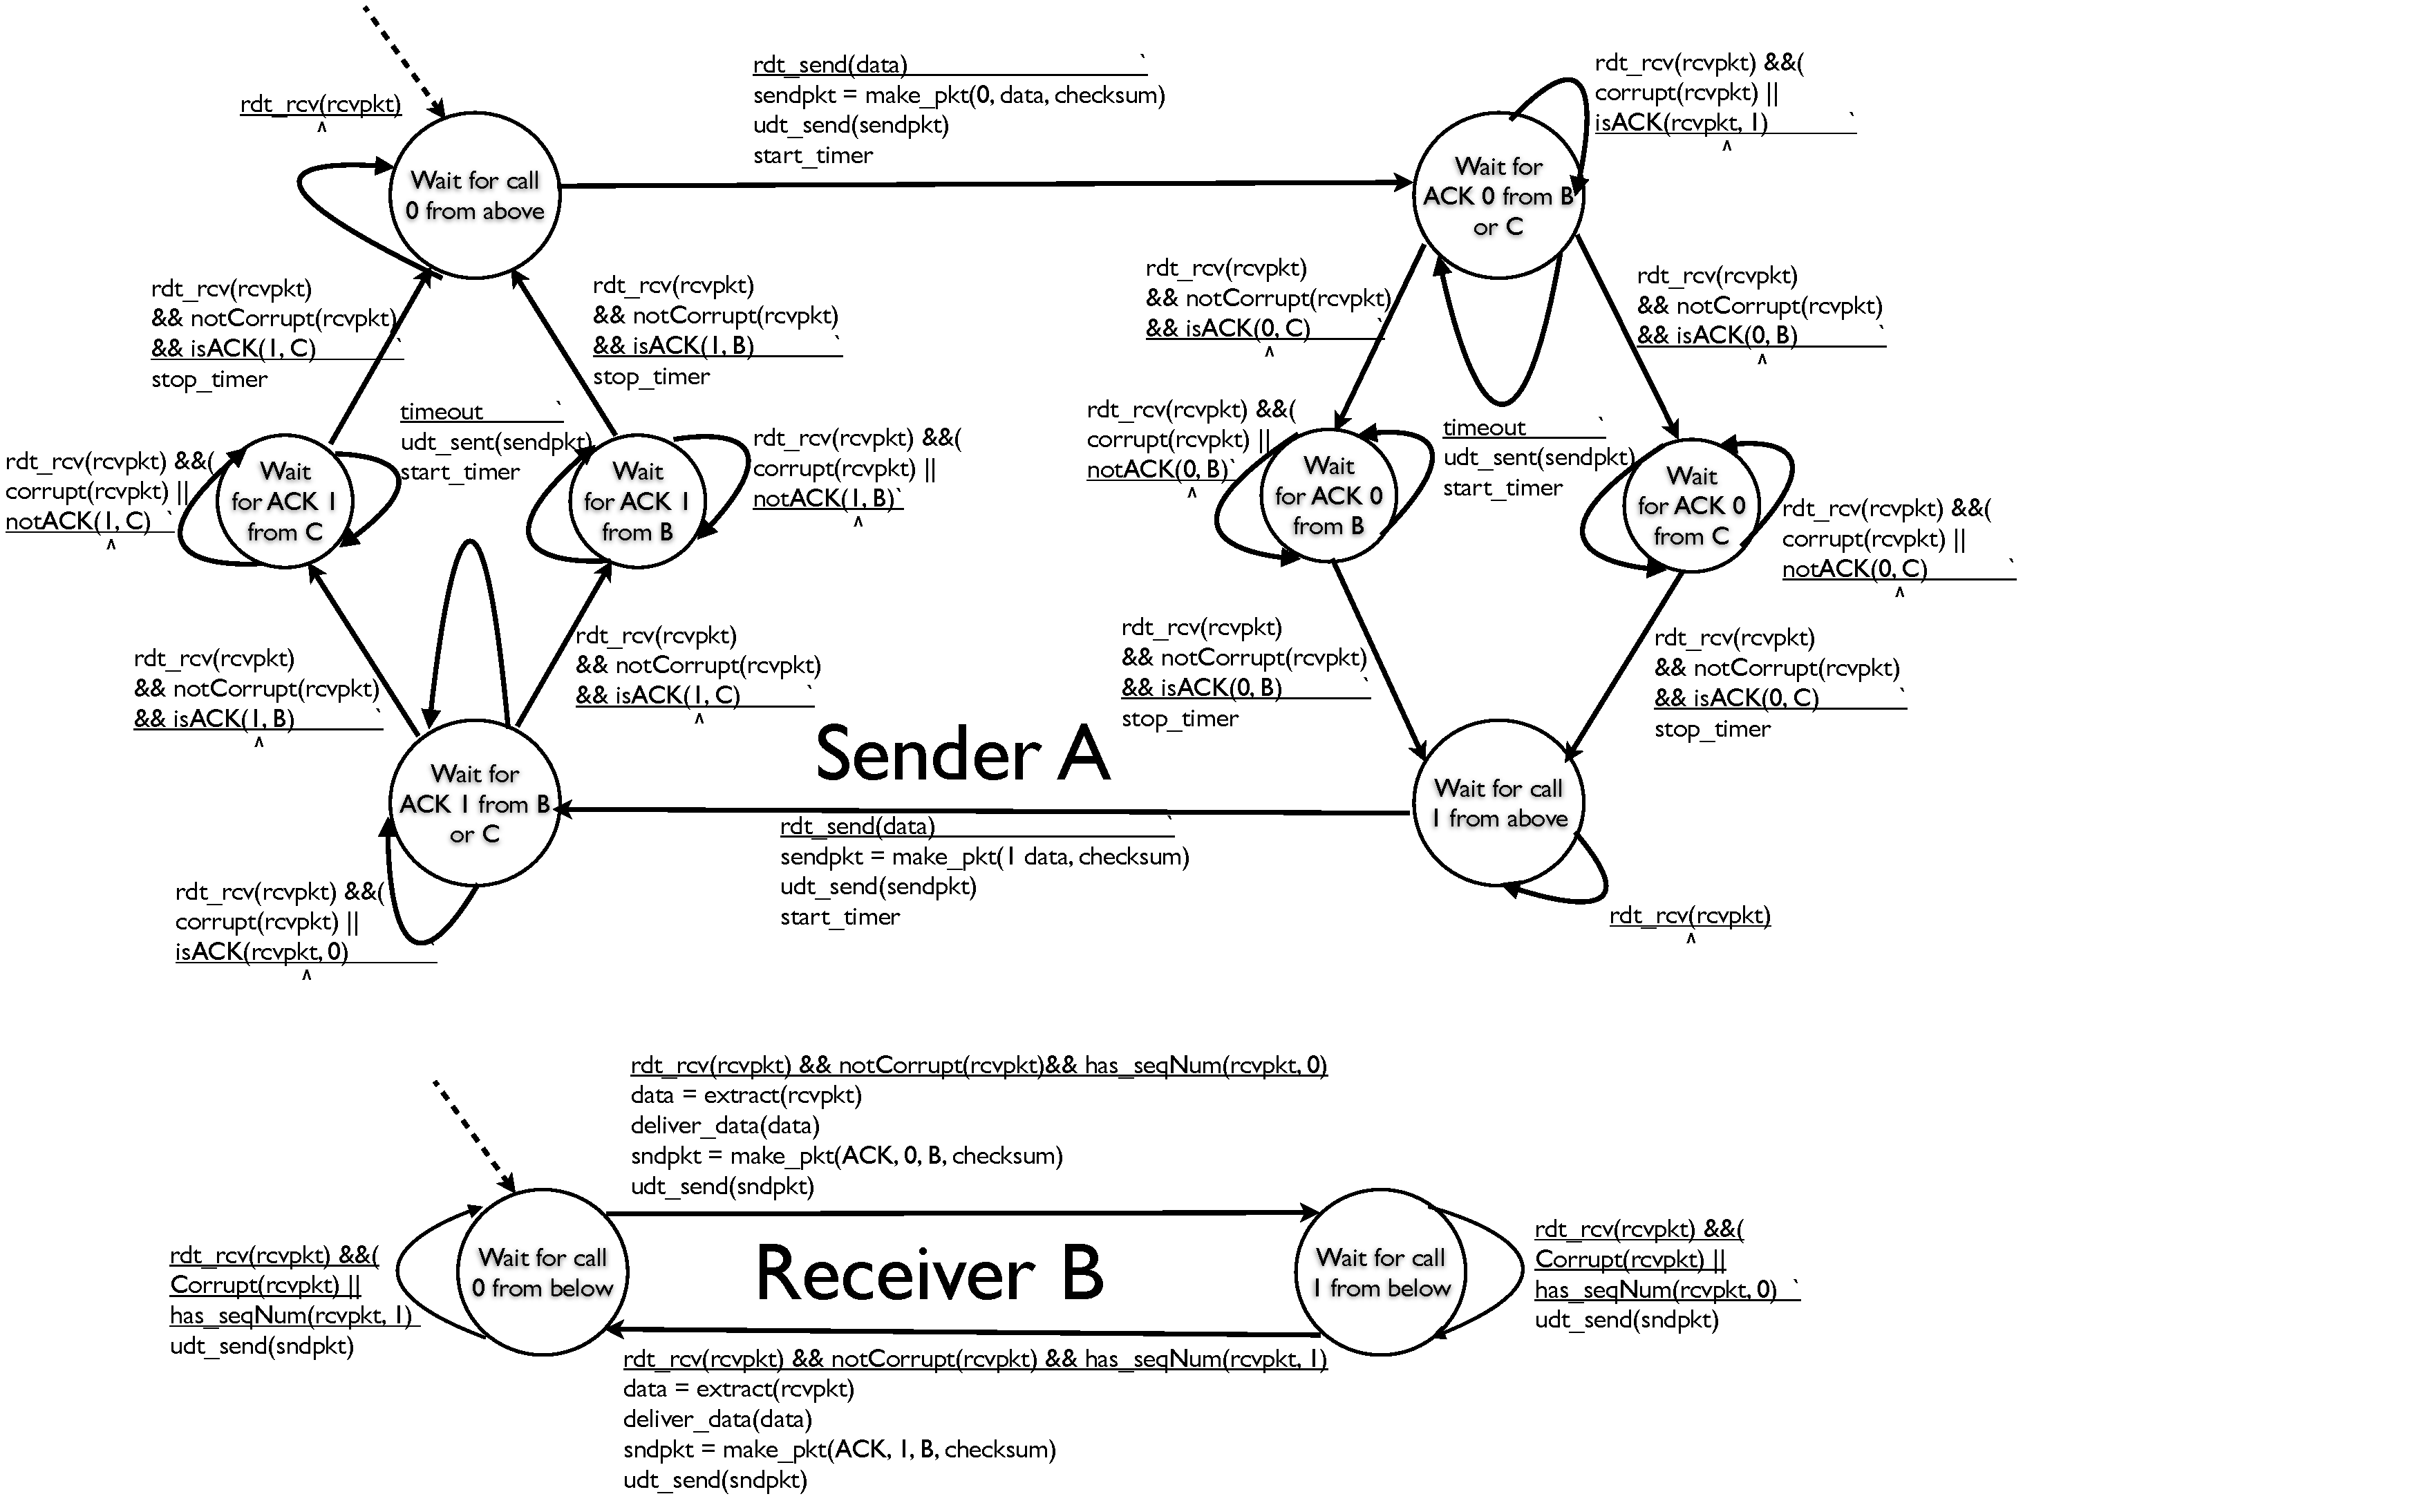
\includegraphics[scale=0.36]{1001.pdf}
The FSM is a variation of rdt 3.0. The squence number of the sending package can
still using the alternating bits (0 and 1). The major difference is that the
sender must receive both ACKs from B and C before ready for listen to the next
available package from its upper layer. Therefore, the "wait for ACK" state will
become three separate states: wait for B or C, wait for B, wait for C, according
to the order of the arrivals of ACKs. Each of the three states will ignore
corrupted or out-of order ACKs. In addtion, ACKs from unanticipated receiver
will also be discarded. Each of the three states waits for ACKs states will
response to a time-out event, when the last made package is retransmitted. 

The receiver side does not vary much from rdt 3.0 except that the package is
supposed to include an identifier to distinguish sending from B or C. 

\pagebreak
\section{Q2}
The AIAD algorithm cannot guarantee the fairness between multiple senders.
Consider the a simple case of two TCP connections sharing a single link with
transmission rate R, as shown in the figure below. Make the same assumptions
as the textbook "assume that the two connections have the same MSS and RTT, and
therefore they have the same congestion window size and the same throughput, and
they have a large amount of data to send, and that no other TCP connections or
UDP datagrams traverse through this shared link. Also, ignore the slow-start
phase of TCP and assume the TCP connections are operating in Congestion
Avoidance mode at all times".

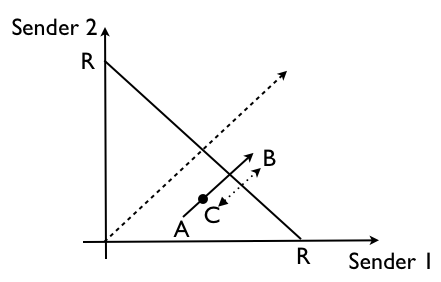
\includegraphics[scale=0.5]{2001.png}

Suppose inititially the allocation point between the two links is at A. Since
the bandwidth has not been fully utilized, with the equal MSS and RTT assumption,
the two links will attempt to increase their window size almost at the same
rate, and therefore, the allocation point will move along the 45 degree link
towards the full bandwidth utilization line. At the first moment that the
allocation point crosses the boundary line, according to the AIAD policy, each
window size will be decrease by a constant. It means that the allocation point B
will slide back to C along the same 45 degree line, and then moves towards the
full utilization line, and so on to continue in an oscillatory way.

In this perspective, the trajectory will never deviate from the line AB, which
is parallel to the equal bandwidth line. In conclusion, unless the initial
allocation point resides on the equal bandwidth line, the bandwidth share will
never be fair among senders.

\pagebreak
\section{Q3}
\subsection{a}
The package total number of packages sent is from the window size of $w/2$ to
$w$, since the window size is incremented by 1 each RTT. Therefore, 
\begin{align}
	N_{sent} &= \frac{w}{2} + \left(\frac{w}{2} + 1 \right) 
		+ \left(\frac{w}{2} + 2\right) + \cdots + w \\
			&= \frac{1}{2}\left(w + \frac{w}{2}\right)
						\left(\frac{w}{2} + 1 \right) \\
			&= \frac{3}{8} w^2 + \frac{3}{4}w
\end{align}
There the loss rate is given,
\begin{align}
	L = \frac{1}{N_{sent}} = \frac{1}{\frac{3}{8} w^2 + \frac{3}{4}w}
\end{align}

\subsection{b}
The data size of each window is MSS and each period contains the number of RTT
equal to that from $\frac{w}{2}$ to $w$, therefore,
\begin{align}
	R &= \frac{ MMS \cdot
		\left( \frac{w}{2} + \left(\frac{w}{2} + 1 \right) 
			+ \left(\frac{w}{2} + 2\right) + \cdots + w 
		\right)
	}{RTT \cdot
		\left( \frac{w}{2} + 1 \right)
		} \\
		&= \frac{3 w}{4} \cdot \frac{MSS}{RTT}
\end{align}
Given that $w^2 \gg w$, 
\begin{align}
	L \approx \frac{1}{\frac{3}{8} w^2} = \frac{8}{3 w^2} 
	\implies w = \sqrt{\frac{3}{8}} \frac{1}{\sqrt{L}}
\end{align}
subtitute it back, 
\begin{align}
	R = \frac{3}{4} \sqrt{\frac{3}{8}} \frac{1}{\sqrt{L}}
		\approx \frac{1.22474 \cdot MSS} {RTT \sqrt{L}}
\end{align}

\section{Q4}
for a) and b) the general formula of the response time for persistent HTTP
connection is, 
\begin{align}
	T_{\text{persistent}}&(RTT, R, BaseSize, ObjectSize) \\
	&= RTT + \left(
				\frac{RTT}{2}
				+ \frac{BaseSize}{R}
				+ \frac{RTT}{2}
			\right) + 
			M \left( 
				\frac{RTT}{2} + 
					\frac{ObjectSize}{R} +
				\frac{RTT}{2} 
			\right) \\
		&= 
			(M + 2) RTT + \frac{1}{R}\left(BaseSize + M \cdot ObjectSize \right)
\end{align}
for non-persistent HTTP connection, 
\begin{align}
	T_{\text{non-persistent}}&(RTT, R, BaseSize, ObjectSize) \\
		&= \left( 2RTT + \frac{BaseSize}{R}\right)
			+ M \times \left( 2RTT + \frac{ObjectSize}{R}\right) \\
		&= 2(M + 1)RTT + \frac{1}{R}\left(BaseSize + M \cdot ObjectSize \right)
\end{align}
\subsection{a}
\begin{center}
Resonse Time with RTT = 100 ms
\vspace{4mm} 

\begin{tabular}{|r|r|r|}
\hline
Bandwith & persistent(s) & non-persistent(s)\\ \hline
28K & 16.91 & 17.91\\ \hline
100K & 5.60 & 6.60\\ \hline
1M & 1.64 & 2.64\\ \hline
10M & 1.24 & 2.24 \\ \hline
\end{tabular}
\vspace{4mm} 

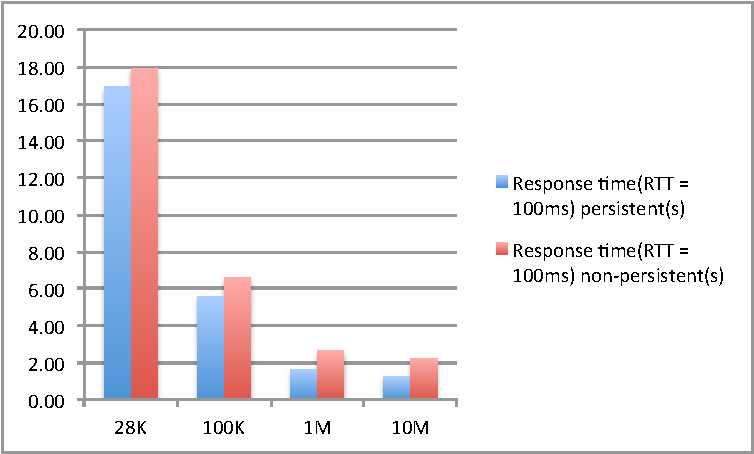
\includegraphics{4a_chart.pdf}
\end{center}

\subsection{b}
\begin{center}
Response Time with RTT = 1 s
\vspace{4mm} 

\begin{tabular}{|r|r|r|}
\hline
Bandwith & persistent(s) & non-persistent(s)\\ \hline
28K & 27.71 & 37.71\\ \hline
100K & 16.40 & 26.40\\ \hline
1M & 12.44 & 22.44\\ \hline
10M & 12.04 & 22.04\\ \hline
\end{tabular}
\vspace{4mm} 

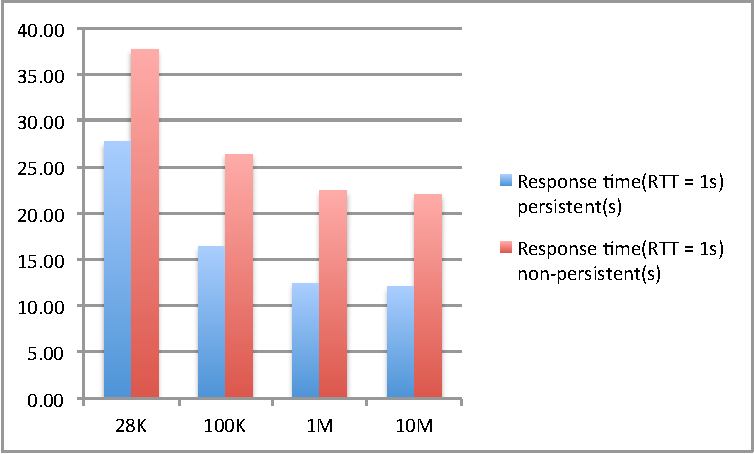
\includegraphics{4b_chart.pdf}
\end{center}

\subsection{c}
For fetching the base page (size=O)
\begin{align}
	T_1 = \frac{RTT}{2} \times 2 + \frac{O}{R} + \frac{RTT}{2} = 2RTT + \frac{O}{R}
\end{align}
For fecthing the objects, at each time point, up to x objects can be download
simultaneously, when the downloading can be interleaving, and therefore there
will $\frac{M}{x}$ sets of simultaneous connections, for each set, 2RTT will be
added in addtion to nodal processing, therefore there will be 
\begin{align}
	T_2 = \frac{M}{x} \times 2RTT + M \times \frac{O}{R}
\end{align}
Given the TCP SSL, the total time is
\begin{align}
	T &= T_1 + T_2 + SSL \\
		&= (M + 1) \frac{O}{R} + 2 \left(\frac{M}{x} + 1 \right)RTT + SSL
\end{align}
\section{Q5}
\subsection{a}
The binary-from IPv4 prefix that CIDR allocated is 
\begin{align}
	200.15.0.0/20 \to 11001000.00001111.0000| 0000.00000000
\end{align}
Since there are six networks supposed to be designed, at least three bits ($2^3
= 8 > 6$) are needed to identify the six networks. The eight subset candidates 
are
\begin{align}
200.15.0.0/23 \to 11001000.00001111.0000000|0.00000000 \\
200.15.2.0/23 \to 11001000.00001111.0000001|0.00000000 \\
200.15.4.0/23 \to 11001000.00001111.0000010|0.00000000 \\
200.15.6.0/23 \to 11001000.00001111.0000011|0.00000000 \\ 
200.15.8.0/23 \to 11001000.00001111.0000100|0.00000000 \\
200.15.10.0/23 \to 11001000.00001111.0000101|0.00000000 \\
200.15.12.0/23 \to 11001000.00001111.0000110|0.00000000 \\
200.15.14.0/23 \to 11001000.00001111.0000111|0.00000000
\end{align}
One possible allocation is labeled in the following graph: (Here we're using the
mid six ones and reserving the first/last one. It's valid to select any six distinct
ones form the above eight subsets.)
\begin{center}
	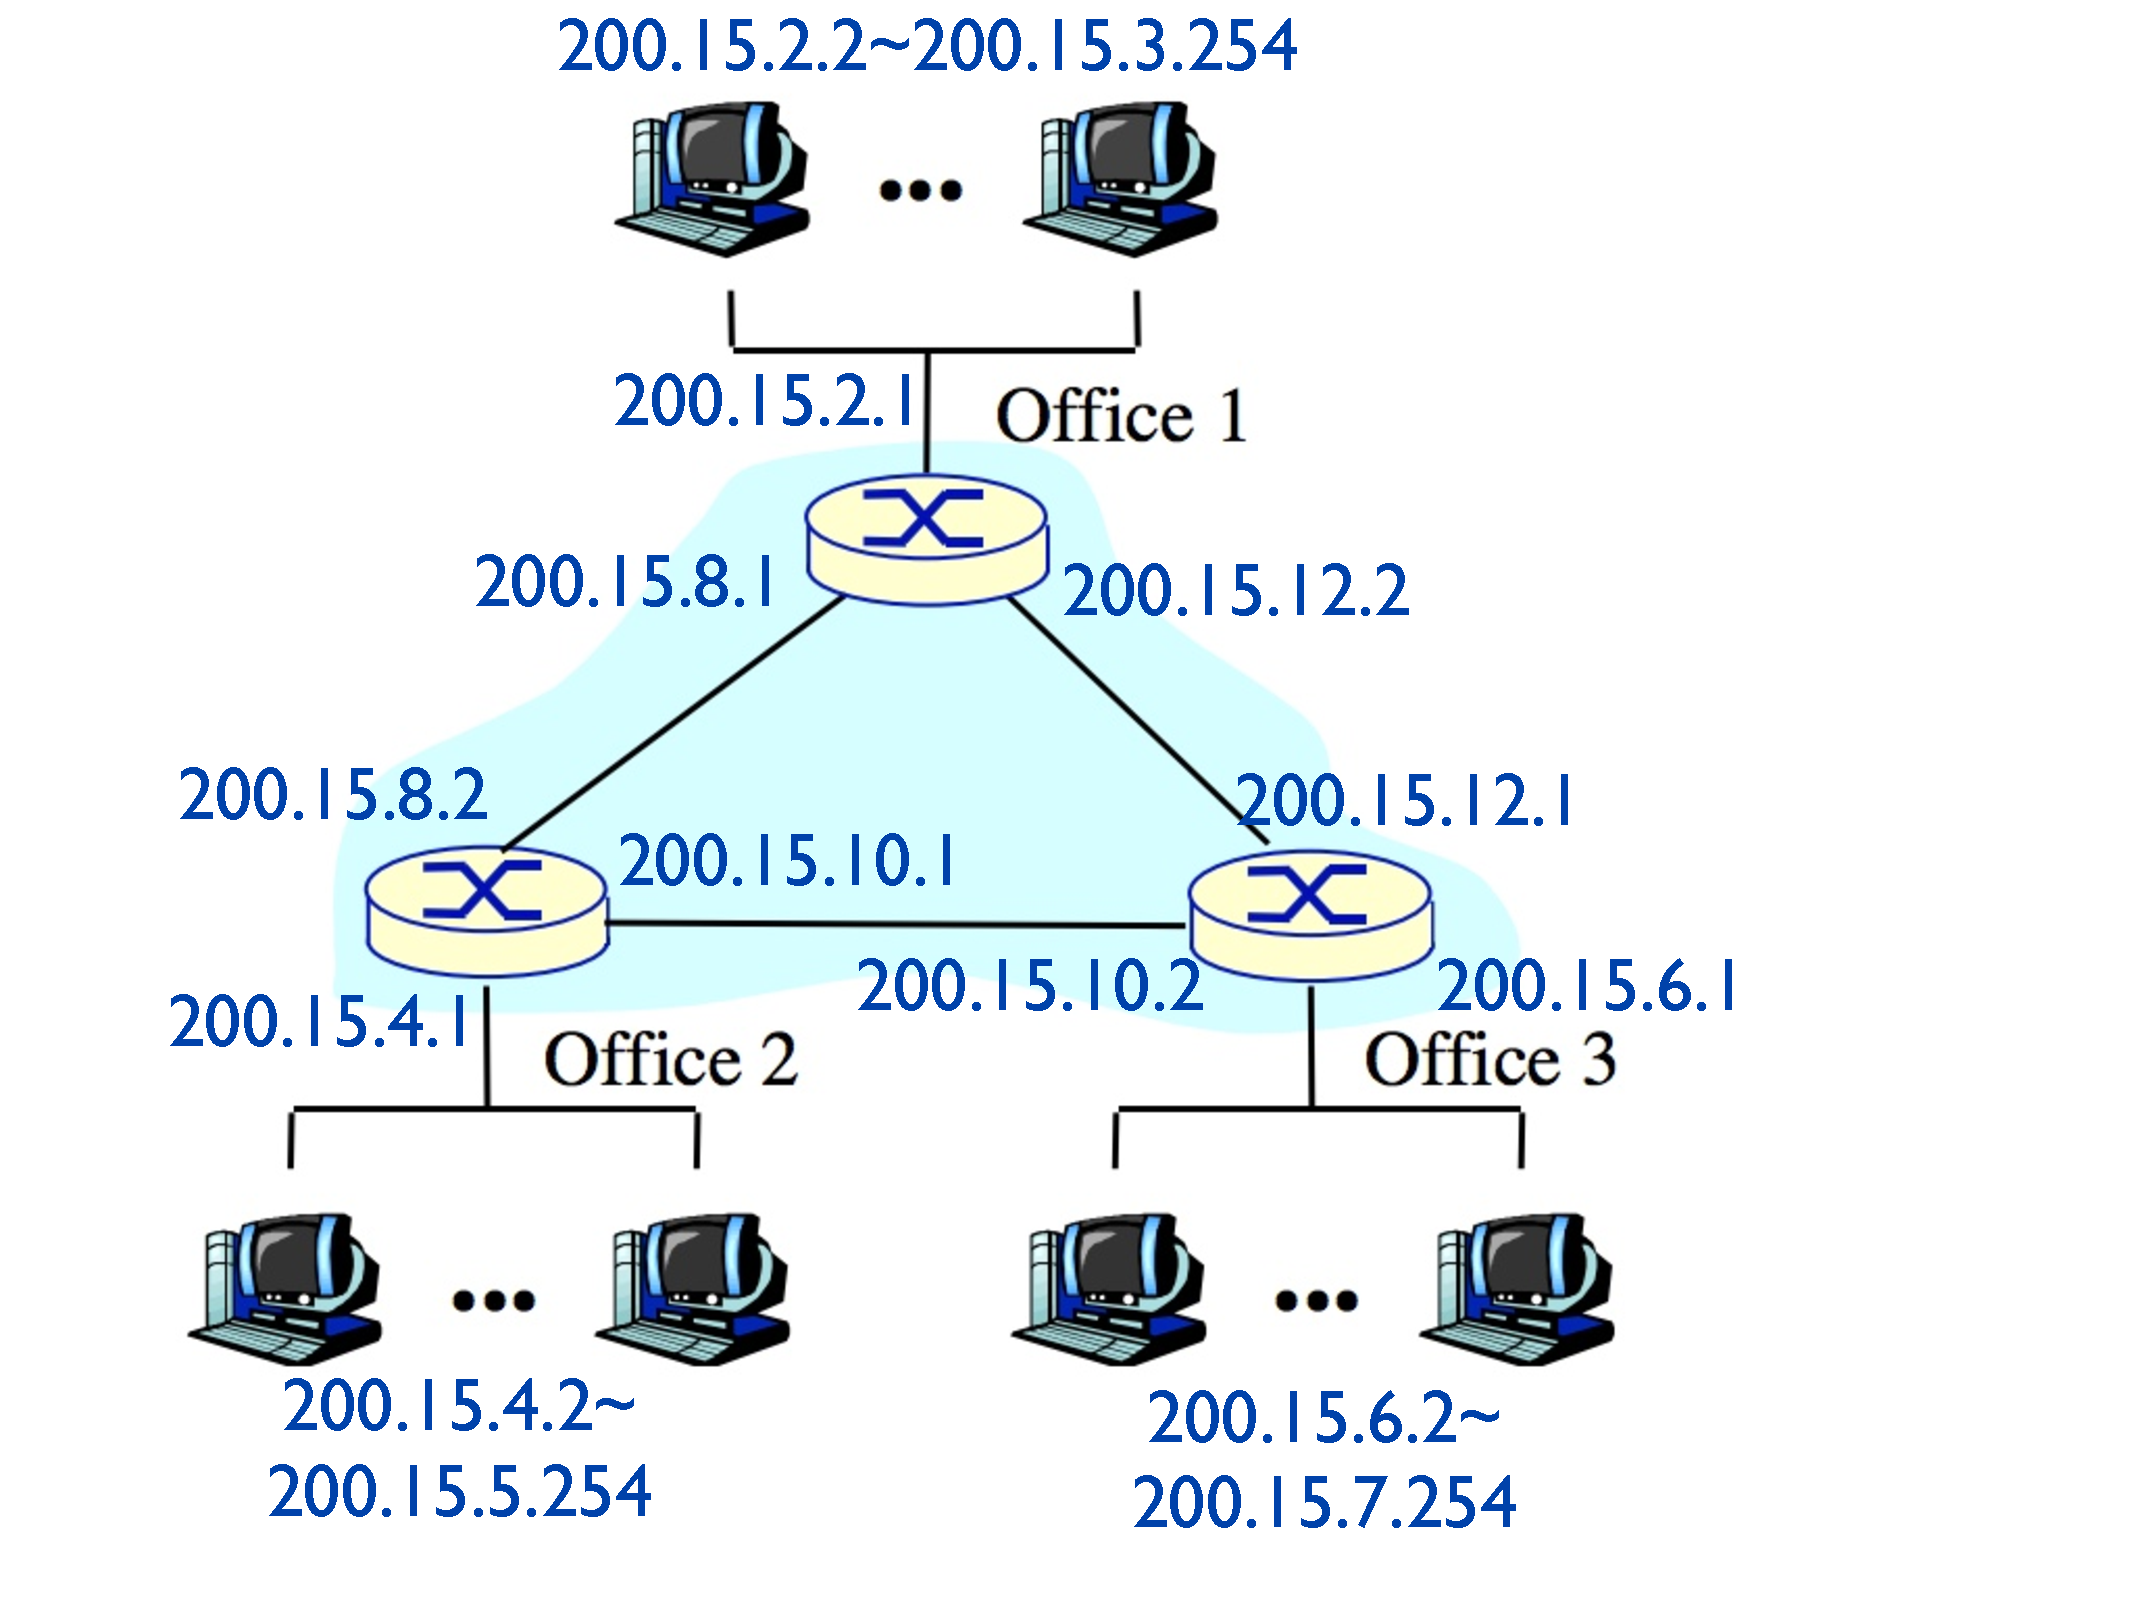
\includegraphics[scale=0.32]{5001.pdf}
\end{center}
For each of the three office locations, the total number capacity of hosts is 
\begin{equation}
	2^9 - 2 = 510 > 300
\end{equation}

\subsection{b}
\begin{center}
	Router in Office 1
	\vspace{4mm}
	
	\begin{tabular}{|c|c|c|c|}
		\hline
		Dest. Network & Next Router & Nhops & interface \\ \hline
		200.15.2.0/23 & - & 1 & 200.15.2.1 \\ \hline
		200.15.4.0/23 & 200.15.8.2 & 2 & 200.15.8.1 \\ \hline
		200.15.6.0/23 & 200.15.12.1 & 2 & 200.15.12.2 \\ \hline
		200.15.8.0/23 & - & 1 & 200.15.12.1 \\ \hline
		200.15.10.1 & 200.15.8.2 & 2 & 200.15.8.1 \\ \hline
		200.15.10.2 & 200.15.12.1 & 2 & 200.15.12.2 \\ \hline
		200.15.12.0/23 & - & 1 & 200.15.12.2 \\ \hline
	\end{tabular}
\end{center}

\begin{center}
	Router in Office 2
	\vspace{4mm}
	
	\begin{tabular}{|c|c|c|c|}
		\hline
		Dest. Network & Next Router & Nhops & interface \\ \hline
		200.15.2.0/23 & 200.15.8.1 & 2 & 200.15.8.2 \\ \hline
		200.15.4.0/23 & - & 1 & 200.15.4.1 \\ \hline
		200.15.6.0/23 & 200.15.10.2 & 2 & 200.15.10.1 \\ \hline
		200.15.8.0/23 & - & 1 & 200.15.8.2 \\ \hline
		200.15.10.0/23 & - & 1 & 200.15.10.1 \\ \hline
		200.15.12.1 & 200.15.10.2 & 2 & 200.15.10.1 \\ \hline
		200.15.12.2 & 200.15.8.1 & 2 & 200.15.8.2 \\ \hline
	\end{tabular}
\end{center}

\begin{center}
	Router in Office 3
	\vspace{4mm}
	
	\begin{tabular}{|c|c|c|c|}
		\hline
		Dest. Network & Next Router & Nhops & interface \\ \hline
		200.15.2.0/23 & 200.15.12.2 & 2 & 200.15.12.1 \\ \hline
		200.15.4.0/23 & 200.15.10.1 & 2 & 200.15.10.2 \\ \hline
		200.15.6.0/23 & -			 & 1 & 200.15.6.1 \\ \hline
		200.15.8.1		& 200.15.12.2 & 2 & 200.15.12.1 \\ \hline
		200.15.8.2		& 200.15.10.1 & 2 & 200.15.10.2 \\ \hline
		200.15.10.0/23 & - & 1 & 200.15.10.2 \\ \hline
		200.15.12.0/23 & - & 1 & 200.15.12.1 \\ \hline
	\end{tabular}
\end{center}

\subsection{c}
\begin{center}
	A typical host in Office 1
	\vspace{4mm}
	
	\begin{tabular}{|c|c|c|}
		\hline
		Dest. Network	&	next router		&	Nhops	\\ \hline
		200.15.2.0/23	&	-	&	1	\\ \hline
		200.15.4.0/23	&	200.15.2.1	&	3	\\ \hline
		200.15.6.0/23	&	200.15.2.1	&	3	\\ \hline
		200.15.8.0/23	&	200.15.2.1	&	2	\\ \hline
		200.15.10.0/23	&	200.15.2.1	&	3	\\ \hline
		200.15.12.0/23	&	200.15.2.1	&	2	\\ \hline
		*(default)	&	200.15.2.1	&	*	\\ \hline
	\end{tabular}
\end{center}

\begin{center}
	A typical host in Office 2
	\vspace{4mm}
	
	\begin{tabular}{|c|c|c|}
		\hline
		Dest. Network	&	next router		&	Nhops	\\ \hline
		200.15.2.0/23	&	200.15.4.1	&	3	\\ \hline
		200.15.4.0/23	&	-			&	1	\\ \hline
		200.15.6.0/23	&	200.15.4.1	&	3	\\ \hline
		200.15.8.0/23	&	200.15.4.1	&	2	\\ \hline
		200.15.10.0/23	&	200.15.4.1	&	2	\\ \hline
		200.15.12.0/23	&	200.15.4.1	&	3	\\ \hline
		*(default)	&	200.15.4.1	&	*	\\ \hline
	\end{tabular}
\end{center}

\begin{center}
	A typical host in Office 3
	\vspace{4mm}
	
	\begin{tabular}{|c|c|c|}
		\hline
		Dest. Network	&	next router		&	Nhops	\\ \hline
		200.15.2.0/23	&	200.15.6.1	&	3	\\ \hline
		200.15.4.0/23	&	200.15.6.1	&	3	\\ \hline
		200.15.6.0/23	&	-			&	1	\\ \hline
		200.15.8.0/23	&	200.15.6.1	&	3	\\ \hline
		200.15.10.0/23	&	200.15.6.1	&	2	\\ \hline
		200.15.12.0/23	&	200.15.6.1	&	2	\\ \hline
		*(default)	&	200.15.6.1	&	*	\\ \hline
	\end{tabular}
\end{center}

\section{Q6}
	Suppose each link cost is measured in time unit, then the message propagates
	as time unit steps. Let the time stamp for the original message is $t=0$ for
	(1) Node C: $C \to D = \infty $ (2) Node D: $D \to C = \infty$.
	\subsection{a}
	The set of message that A received are
	\vspace{4mm}
	
	\begin{tabular}{|c|c|c|c|c|c|}
		\hline
		t & 1 & 3 & 4 & 5 & 7 \\ \hline
		msg & 
		$D \to C = \infty $ & 
		$C \to D = \infty$  & 
		$D \to C = \infty$ & 
		$	
				C \to D = \infty,
				C \to D = \infty 
		$ & 
		$D \to C = \infty$\\
		\hline
	\end{tabular}
	
	\subsection{b}
	The corresponding actions take by A:
	\vspace{4mm}
	
	\begin{tabular}{|c|c|c|}
		\hline
		t & Msg Received & Action \\ \hline
		1 & $D \to C = \infty $	& update local data and forward\\ \hline
		3 & $C \to D = \infty $	& update local data and forward\\ \hline
		4 & $D \to C = \infty $	& ignore the message\\ \hline
		5 & $C \to D = \infty $	& ignore the message \\ \hline
		5 & $C \to D = \infty $	& ignore the message \\ \hline
		7 & $D \to C = \infty $	& ignore the message \\ \hline
	\end{tabular}
	
\section{Q7}
	Let the topology of the network be a graph with finite nodes connected by
	finite undirectly-weighted edges.  
	
	In the scenario of initially building the routing table, let $L_{max\_hops}$ be
	the longest possible path without a loop. The value obviously exists due the finite
	property of the graph. Measured in edge count without considering the edge
	weight, presumably $|L_{max\_hops}|< $ total number of edges. Since the
	question make the assumption of synchronous updates, suppose one period of
	iteration is each node delivers its distance vector to all its neighbours. Then
	after $|L_{max\_hops}|-1 $ iterations, all nodes will get the inforamtion the
	shortest path cost of up to $|L_{max\_hops}|-1 $ hops to all other nodes. Any
	path with $|L_{max\_hops}|$ more hops will result in loops, which is more costy
	than the loop-free path, therefore the algorithm will converge in at most
	$|L_{max\_hops}|-1 $ interations. 
	
	In the case of a link cost change, it may not guarantee the algorithm
	terminates in finite steps if some link cost increases to infinity (an edge
	breaks up). It's subject to the count-to-infinity problem, when the some
	distance will "converge to infinity" as the algorithm goes. 
	
\section{Q8}
\subsection{a}
	\begin{multicols}{2}
	
	\begin{itemize}
	\item Router A: 
		\begin{itemize}
		  \item to B: 19.8.0.1/30
		  \item to C: 19.8.0.14/30
		  \item to intra: 152.2.131.1/24
		\end{itemize}
	\item Router B: 
		\begin{itemize}
		  \item to A: 19.8.0.2/30; 
		  \item to D: 19.8.0.5/30; 
		  \item to intra: 168.6.192.1/20
		\end{itemize}
	\item Router C: 
		\begin{itemize}
		  \item to A: 19.8.0.13/30; 
		  \item to D: 19.8.0.10/30; 
		  \item to intra: 200.12.96.1/20
		\end{itemize}
	\item Router D: 
		\begin{itemize}
		  \item to B: 19.8.0.6/30; 
		  \item to C: 19.8.0.9/30; 
		  \item to intra: 223.127.224.1/20
		\end{itemize}
	\end{itemize}
	
	\columnbreak
		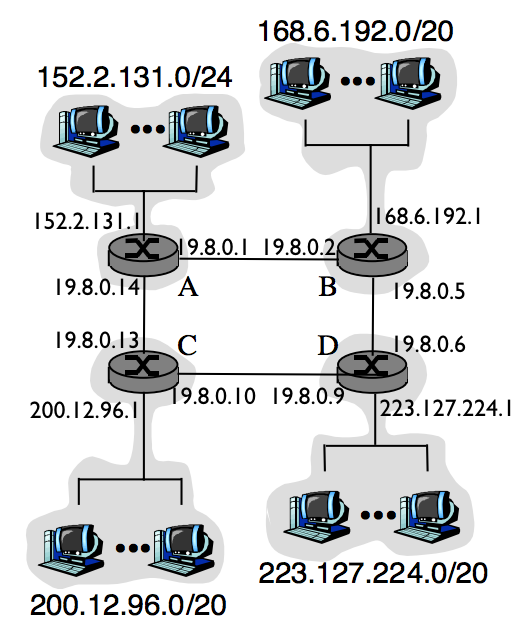
\includegraphics[scale=0.35]{8001.png}
	\end{multicols}
	
\subsection{b}
	\begin{center}
		Router A \\
		\vspace{2mm}
		
		\begin{tabular}{|c|c|c|c|}
			\hline
			Dest. Network  & Next Router & Nhops & interface\\ 
			\hline
				152.2.131.0/24 & - & 1 & 152.2.131.1\\
				168.6.192.0/20 & 19.8.0.2 & 2 & 19.8.0.1\\ 
				200.12.96.0/20 & 19.8.0.13 & 2 & 19.8.0.14\\ 
				223.127.224.0/20 & 19.8.0.2 & 3 & 19.8.0.1\\ 
				19.8.0.0/30 & - & 1 & 19.8.0.1\\ 
				19.8.0.4/30 & 19.8.0.2 & 2 & 19.8.0.1\\ 
				19.8.0.8/30 & 19.8.0.13 & 2 & 19.8.0.14\\ 
				19.8.0.12/30 & - & 1 & 19.8.0.14 \\
			\hline
		\end{tabular}
	\end{center}

	\begin{center}
		Router B \\
		\vspace{2mm}
		
		\begin{tabular}{|c|c|c|c|}
			\hline
			Dest. Network  & Next Router & Nhops & interface\\ 
			\hline
				152.2.131.0/24 & 19.8.0.1 & 2 & 19.8.0.2\\ 
				168.6.192.0/20 & - & 1 & 168.6.192.1\\ 
				200.12.96.0/20 & 19.8.0.6 & 3 & 19.8.0.5\\ 
				223.127.224.0/20 & 19.8.0.6 & 2 & 19.8.0.5\\ 
				19.8.0.0/30 & - & 1 & 19.8.0.2\\ 
				19.8.0.4/30 & - & 1 & 19.8.0.5\\ 
				19.8.0.8/30 & 19.8.0.6 & 2 & 19.8.0.5\\ 
				19.8.0.12/30 & 19.8.0.1 & 2 & 19.8.0.2\\
			\hline
		\end{tabular}
	\end{center}

	\begin{center}
		Router C \\
		\vspace{2mm}
		
		\begin{tabular}{|c|c|c|c|}
			\hline
			Dest. Network  & Next Router & Nhops & interface\\ 
			\hline
				152.2.131.0/24 & 19.8.0.14 & 2 & 19.8.0.13\\ 
				168.6.192.0/20 & 19.8.0.14 & 3 & 19.8.0.13\\ 
				200.12.96.0/20 & - & 1 & 200.12.96.1\\ 
				223.127.224.0/20 & 19.8.0.10 & 2 & 19.8.0.9\\ 
				19.8.0.0/30 & 19.8.0.14 & 2 & 19.8.0.13\\ 
				19.8.0.4/30 & 19.8.0.9 & 2 & 19.8.0.10\\ 
				19.8.0.8/30 & - & 1 & 19.8.0.10\\ 
				19.8.0.12/30 & - & 1 & 19.8.0.13\\
			\hline
		\end{tabular}
	\end{center}

	\begin{center}
		Router D \\
		\vspace{2mm}
		
		\begin{tabular}{|c|c|c|c|}
			\hline
			Dest. Network  & Next Router & Nhops & interface\\ 
			\hline
				152.2.131.0/24 & - & 3 & 19.8.0.9\\ 
				168.6.192.0/20 & 19.8.0.5 & 2 & 19.8.0.6\\ 
				200.12.96.0/20 & 19.8.0.10 & 2 & 19.8.0.9\\ 
				223.127.224.0/20 & 19.8.0.2 & 1 & 223.127.224.1\\ 
				19.8.0.0/30 & 19.8.0.5 & 2 & 19.8.0.6\\ 
				19.8.0.4/30 & - & 1 & 19.8.0.6\\ 
				19.8.0.8/30 & - & 1 & 19.8.0.9\\ 
				19.8.0.12/30 & 19.8.0.10 & 2 & 19.8.0.9 \\
			\hline
		\end{tabular}
	\end{center}

	\begin{center}
		A Host in AS-A \\
		\vspace{2mm}
		
		\begin{tabular}{|c|c|c|}
			\hline
			Dest. Network  & Next Router & Nhops\\ 
			\hline
				152.2.131.0/24 & - & 1\\ 
				168.6.192.0/20 & 152.2.131.1 & 3\\ 
				200.12.96.0/20 & 152.2.131.1 & 3\\ 
				223.127.224.0/20 & 152.2.131.1 & 4\\ 
				19.8.0.0/30 & 152.2.131.1 & 2\\ 
				19.8.0.4/30 & 152.2.131.1 & 3\\ 
				19.8.0.8/30 & 152.2.131.1 & 3\\ 
				19.8.0.12/30 & 152.2.131.1 & 2\\ 
				(*default) & 152.2.131.1 & * \\
			\hline
		\end{tabular}
	\end{center}

	\begin{center}
		A Host in AS-B \\
		\vspace{2mm}
		
		\begin{tabular}{|c|c|c|}
			\hline
			Dest. Network  & Next Router & Nhops\\ 
			\hline
				152.2.131.0/24 & 168.6.192.1 & 3\\ 
				168.6.192.0/20 & - & 1\\ 
				200.12.96.0/20 & 168.6.192.1 & 4\\ 
				223.127.224.0/20 & 168.6.192.1 & 3\\ 
				19.8.0.0/30 & 168.6.192.1 & 2\\ 
				19.8.0.4/30 & 168.6.192.1 & 2\\ 
				19.8.0.8/30 & 168.6.192.1 & 3\\ 
				19.8.0.12/30 & 168.6.192.1 & 3\\ 
				(*default) & 168.6.192.1 & *\\
			\hline
		\end{tabular}
	\end{center}

	\begin{center}
		A Host in AS-C \\
		\vspace{2mm}
		
		\begin{tabular}{|c|c|c|}
			\hline
			Dest. Network  & Next Router & Nhops\\ 
			\hline
				152.2.131.0/24 & 200.12.96.1 & 3\\ 
				168.6.192.0/20 & 200.12.96.1 & 4\\ 
				200.12.96.0/20 & - & 1\\ 
				223.127.224.0/20 & 200.12.96.1 & 3\\ 
				19.8.0.0/30 & 200.12.96.1 & 3\\ 
				19.8.0.4/30 & 200.12.96.1 & 3\\ 
				19.8.0.8/30 & 200.12.96.1 & 2\\ 
				19.8.0.12/30 & 200.12.96.1 & 2\\ 
				(*default) & 200.12.96.1 & *\\
			\hline
		\end{tabular}
	\end{center}

	\begin{center}
		A Host in AS-D \\
		\vspace{2mm}
		
		\begin{tabular}{|c|c|c|}
			\hline
			Dest. Network  & Next Router & Nhops\\ 
			\hline
				152.2.131.0/24 & 223.127.224.1 & 4\\ 
				168.6.192.0/20 & 223.127.224.1 & 3\\ 
				200.12.96.0/20 & 223.127.224.1 & 3\\ 
				223.127.224.0/20 & - & 1\\ 
				19.8.0.0/30 & 223.127.224.1 & 3\\ 
				19.8.0.4/30 & 223.127.224.1 & 2\\ 
				19.8.0.8/30 & 223.127.224.1 & 2\\ 
				19.8.0.12/30 & 223.127.224.1 & 3\\ 
				(*default) & 223.127.224.1 & *\\
			\hline
		\end{tabular}
	\end{center}


\subsection{c}
	Suppose the four autonomous systems connected with the router A, B, C, D are
	labeled as AS-A(152.2.131.0/24), AS-B(168.6.192.0/20), AS-C(200.12.96.0/20),
	AS-D(223.127.224.0/20), respectively. Also the inter-router subnets are
	AB(19.8.0.0/30), BD(19.8.0.4/30), CD(19.8.0.8/30), AC(19.8.0.12/30). In the BGP
	session, it follows the following principle.
	
	B advertises to D that it has no path to any other destination except for AS-B
	along with four inter-router networks. i.e. B will send to D an advertisement
	with entries - (prefix: 168.9.192.0/20; AS-PATH: AS-B; NEXT-HOP: 19.8.0.5),
	along with the inter-router netwroks AB, BD, CD, AC, which suggests to D is a
	gateway router only connected to a stub network (AS-B) and the four
	inter-router networks. 
	
	In a symmetric sense, D advertises to B that it has no path to a destination
	other than AS-D. i.e. B will send to D an advertisement with entries (prefix:
	223.127.224.4/20; AS-PATH: AS-D; NEXT-HOP: 19.8.0.6), along with the four
	inter-router networks(AB, BD, CD, AC). Therefore, provided the information from
	D, B could infer router D only connects an stub network AS-D as well as
	inter-router networks. When B forwards datagram to A or C, it won't select D
	as a next-hop candidate, since it has no knowledge that AS-A or AS-C is
	reachable via D according to D's advertisement.
	
\end{document}
